%%%%%%%%%%%%%%%%%%%%%%%%%%%%%%%%%%%%%%%%%%%%%%
%Lab report writeup based on template by Derek Hildreth
%%%%%%%%%%%%%%%%%%%%%%%%%%%%%%%%%%%%%%%%%%%%%%

\documentclass[aps,letterpaper,10pt]{article}

\usepackage{graphicx} % For images
\usepackage{float}    % For tables and other floats
\usepackage{verbatim} % For comments and other
\usepackage{amsmath}  % For math
\usepackage{amssymb}  % For more math
\usepackage{fullpage} % Set margins and place page numbers at bottom center
\usepackage{subfig}   % For subfigures
\usepackage[usenames,dvipsnames]{color} % For colors and names
\usepackage{fancyhdr} %headers
\usepackage{wrapfig} % for inline images

\usepackage{easytable}

%%%%%%%%%%%%

%HEADER FORMATING%%%%%%%%%%%%%
\pagestyle{fancy}
\headheight 23pt
\setlength{\headsep}{20pt}
\lhead{18.369 - PSet 4}
\chead{Due 28 March 2016}
\rhead{A.G. Athanassiadis}
%%%%%%%%%%%%%%%%%%%%%%%%

%Custom Definitions%%%%%%%%%%%%%%%
\newcommand{\ttt}{\texttt}
\newcommand{\D}[1]{ $D^{(#1)}$ }
%%%%%%%%%%%%%%%%%%%%%%%%

\begin{document}

\section{Problem 3}

\subsection{Part a}
\begin{figure*}[!h]
\centering
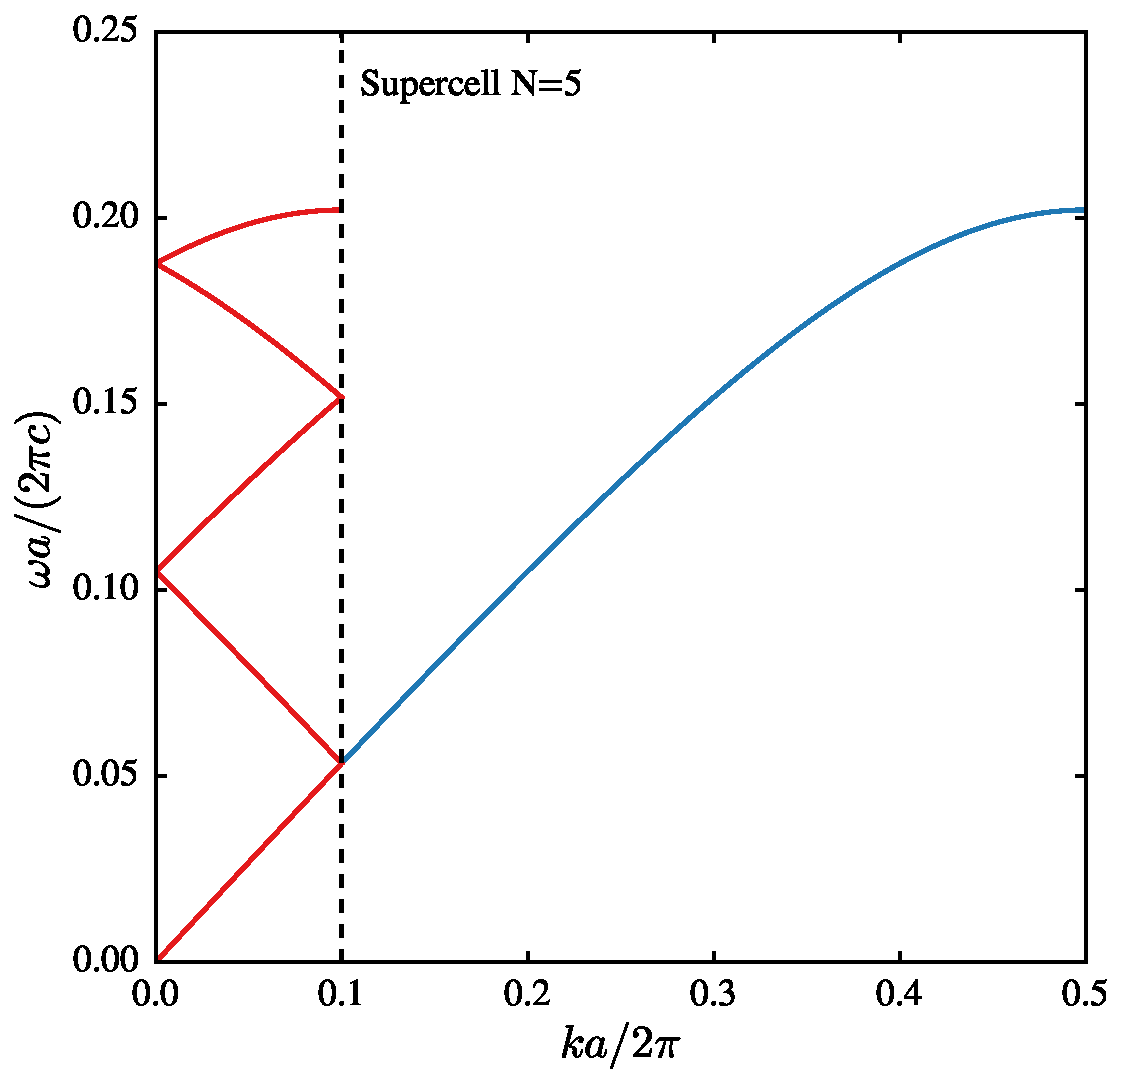
\includegraphics[width=0.5\textwidth]{3a-1}
\caption{\label{fig:3a} The band diagram $\omega(k)$ for a periodic structure of period $a$. The blue curve represents the band calculated in MPB with a single period geometry. The red band represents the band for the same geometry, but repeated in an $N=5$ supercell. As expected, the frequencies fold over when they reach $k=2\pi N / a.$ }
\end{figure*}

\subsection{Part b}
\begin{figure*}[!h]
\centering
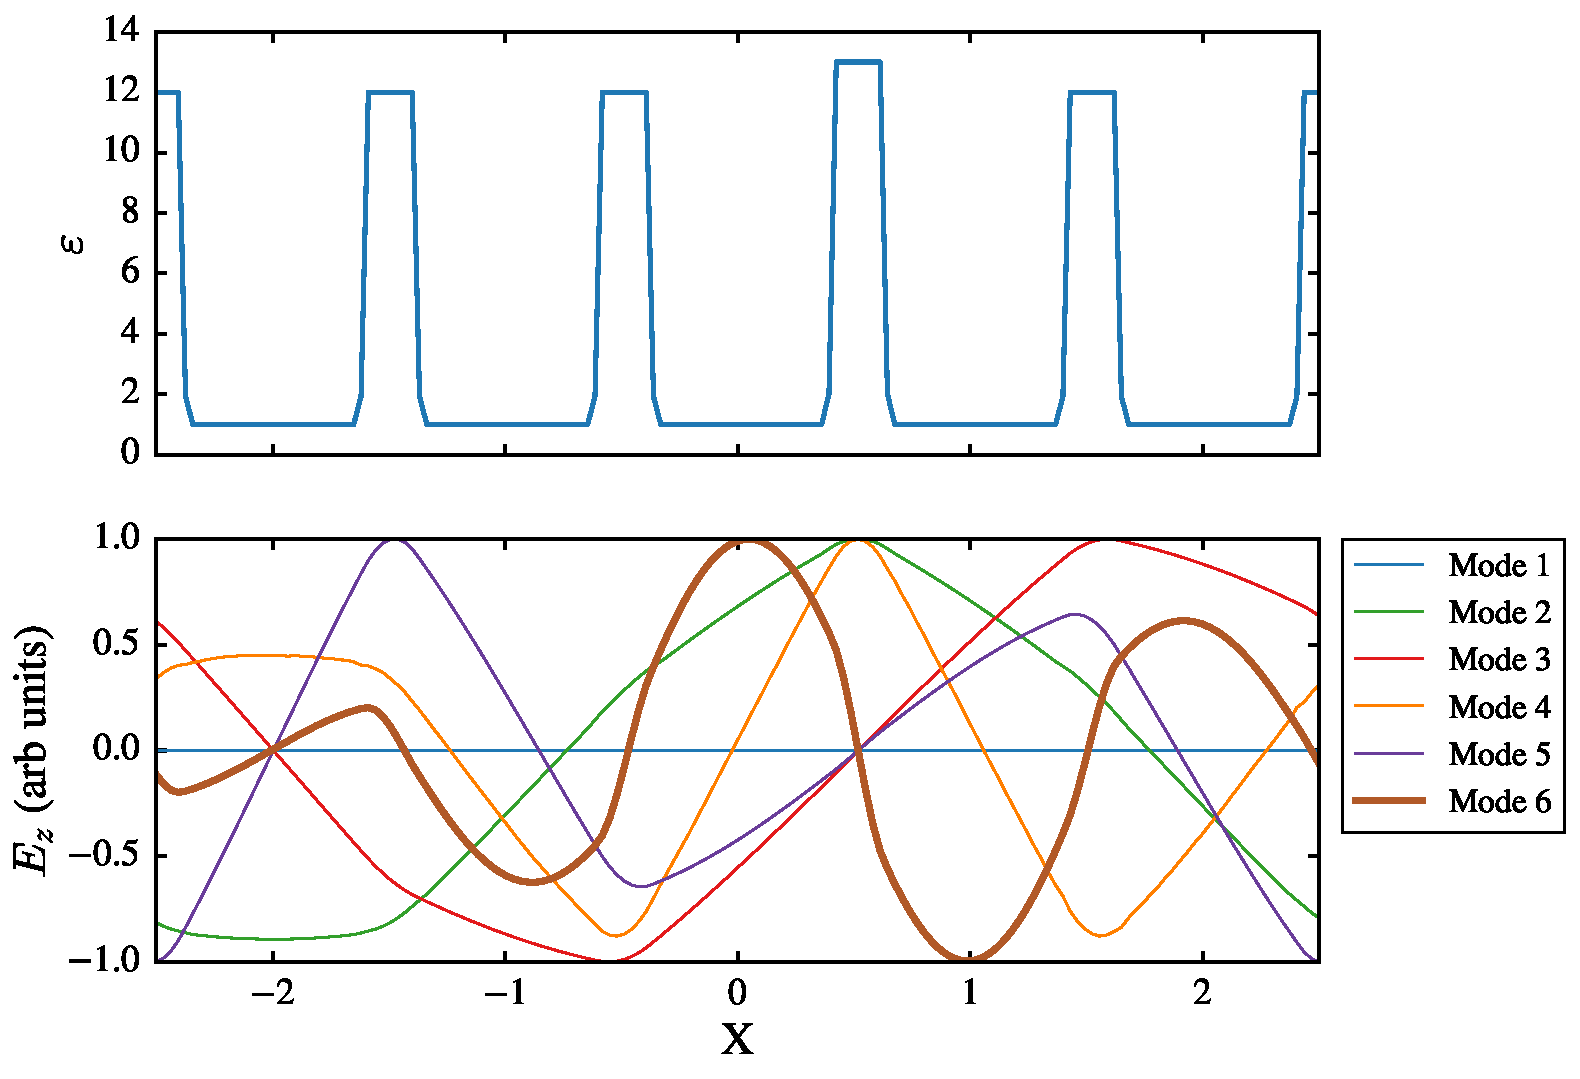
\includegraphics[width=0.48\textwidth]{3b-1}
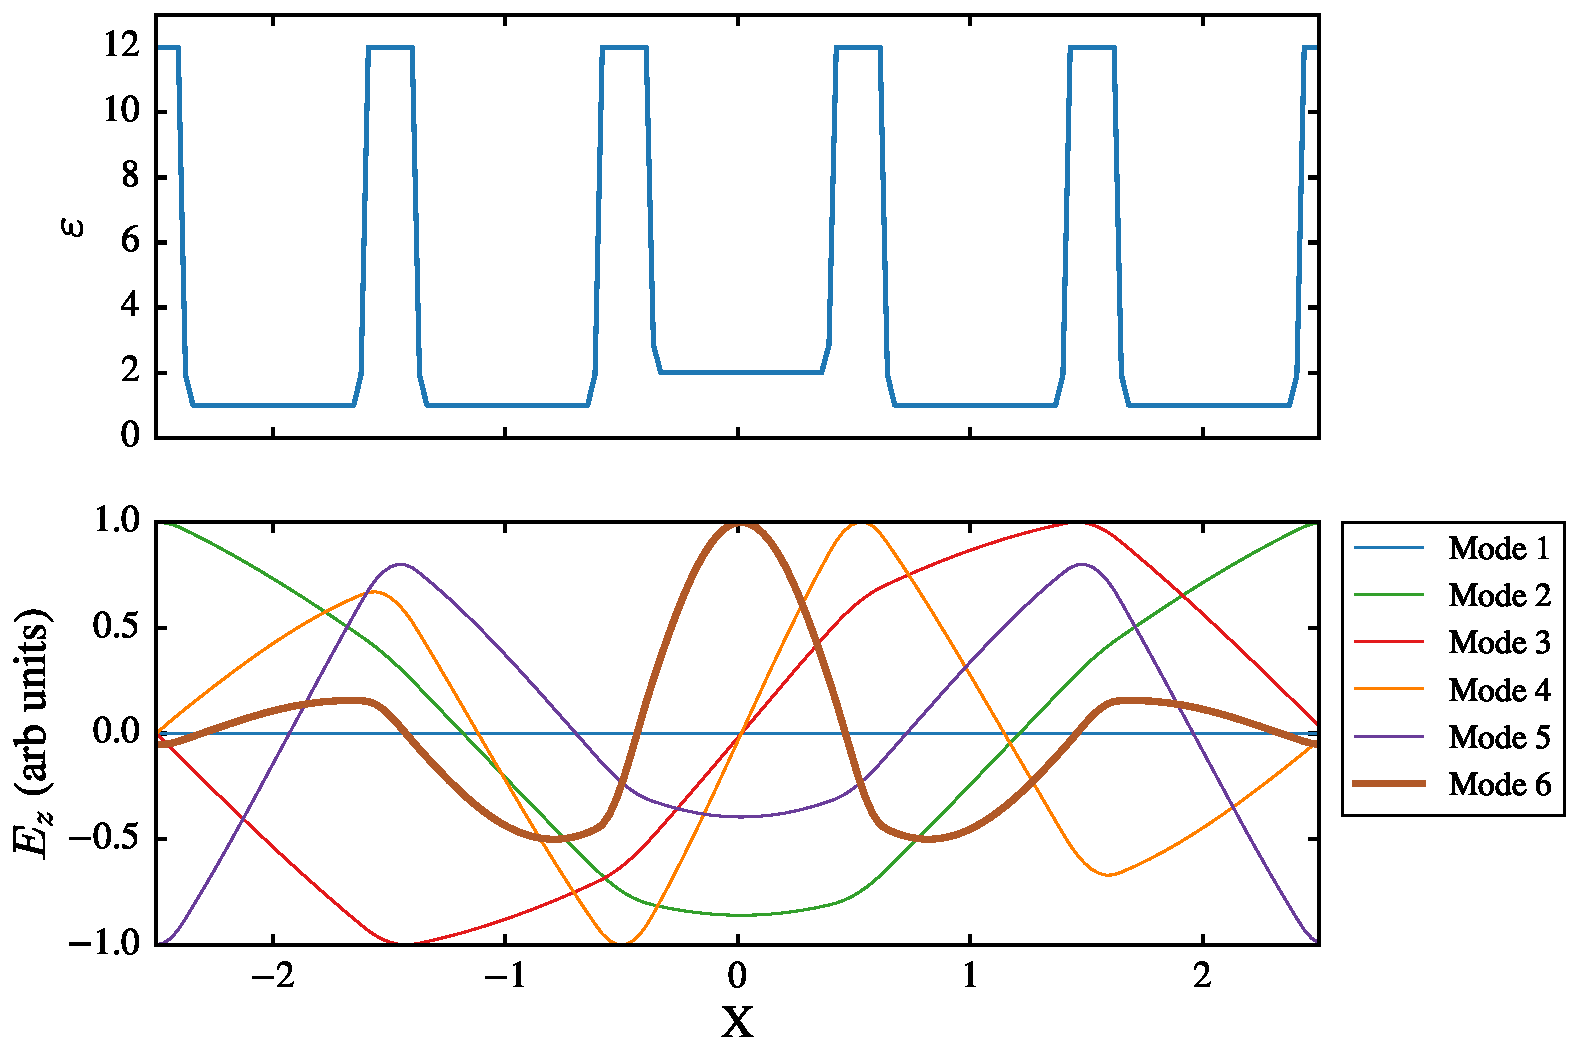
\includegraphics[width=0.48\textwidth]{3b-2}
\caption{\label{fig:3b} $E_z$-fields for different defect modes. (Left) defect in $\varepsilon_1$ (high) - Modes 2 and 4 are even; 3,5 are odd. Mode 6 is odd and decays (it is a localized mode). (Right) defect in $\varepsilon_2$ (low value) - Modes 2 and 5 are even; 3 and 4 are odd; again mode 6 is a localized mode (even) that decays away from the defect. }
\end{figure*}

\subsection{Part c}

\begin{figure*}[!h]
\centering
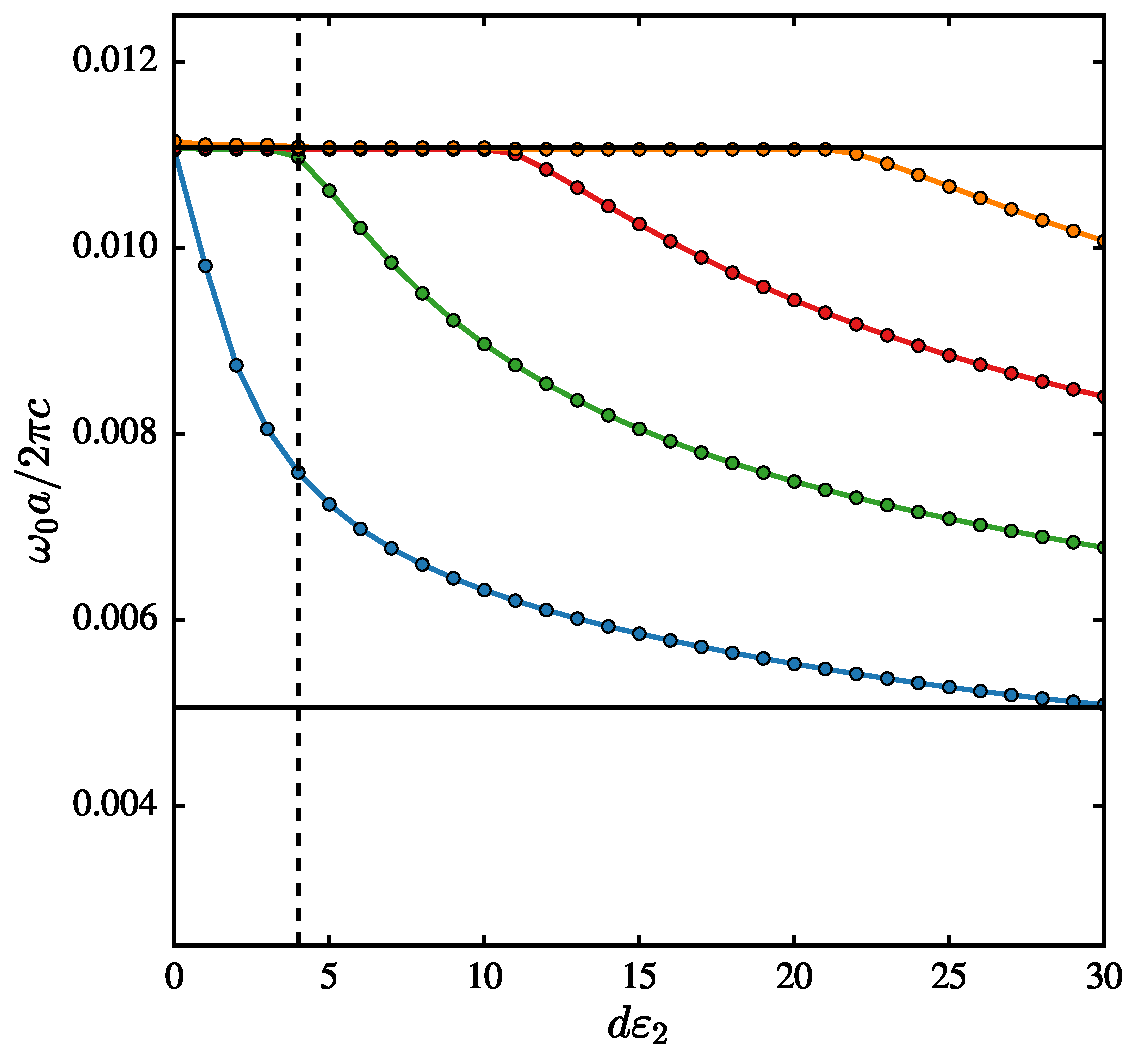
\includegraphics[width=0.48\textwidth]{3c-1}
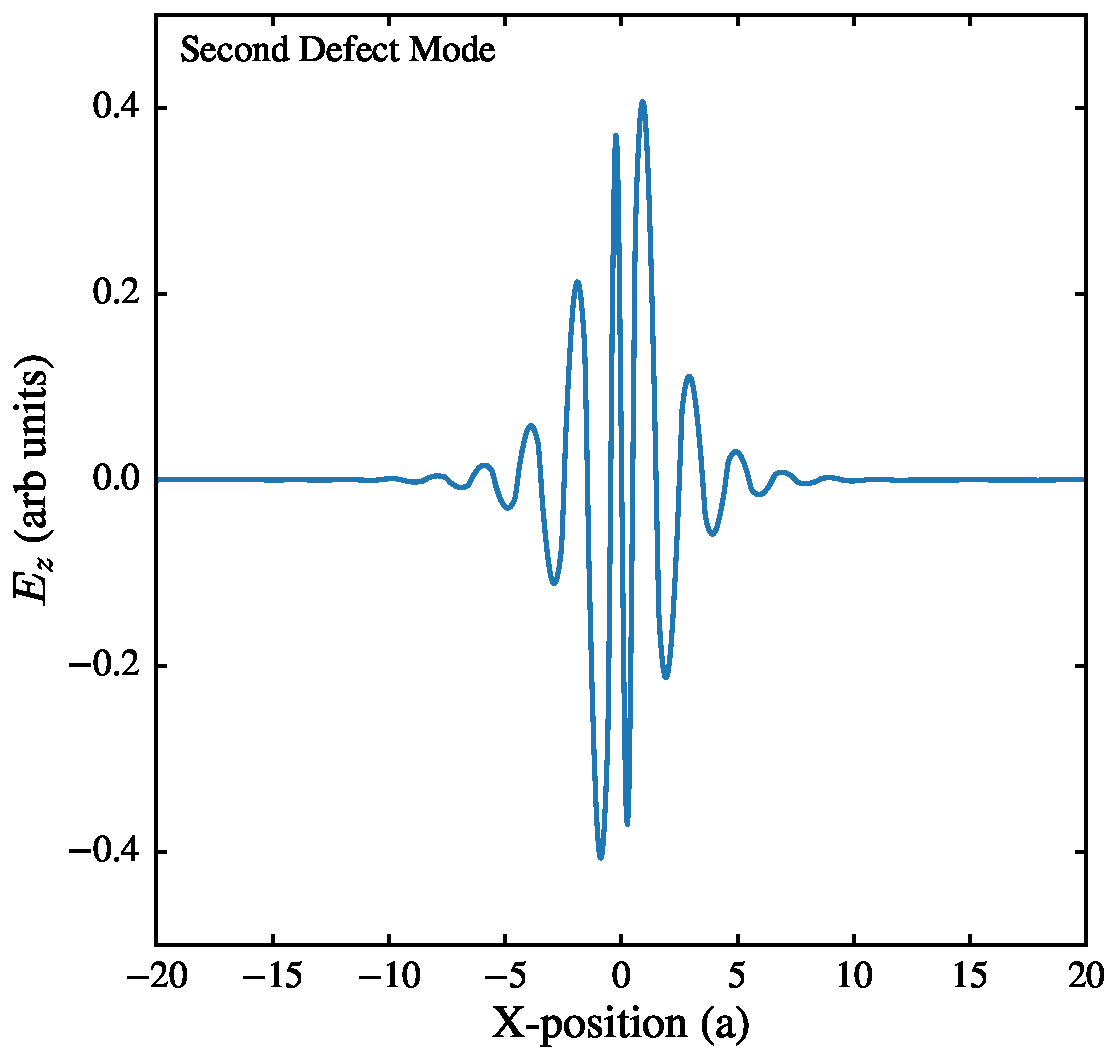
\includegraphics[width=0.48\textwidth]{3c-2}
\caption{\label{fig:3c} (Left) Defect mode frequencies (at $k=0$) within the gap as $\varepsilon_2$ is increased by $d\varepsilon_2$. Solid black lines on the top and bottom indicate the band gap edges for the unperturbed 1d-crystal. A second defect appears when $d\varepsilon_2\approx4.$ (Right) The (localized) electric field for the second defect mode when $d\varepsilon_2=5$. }
\end{figure*}

\subsection{Part d}
\begin{figure*}[!h]
\centering
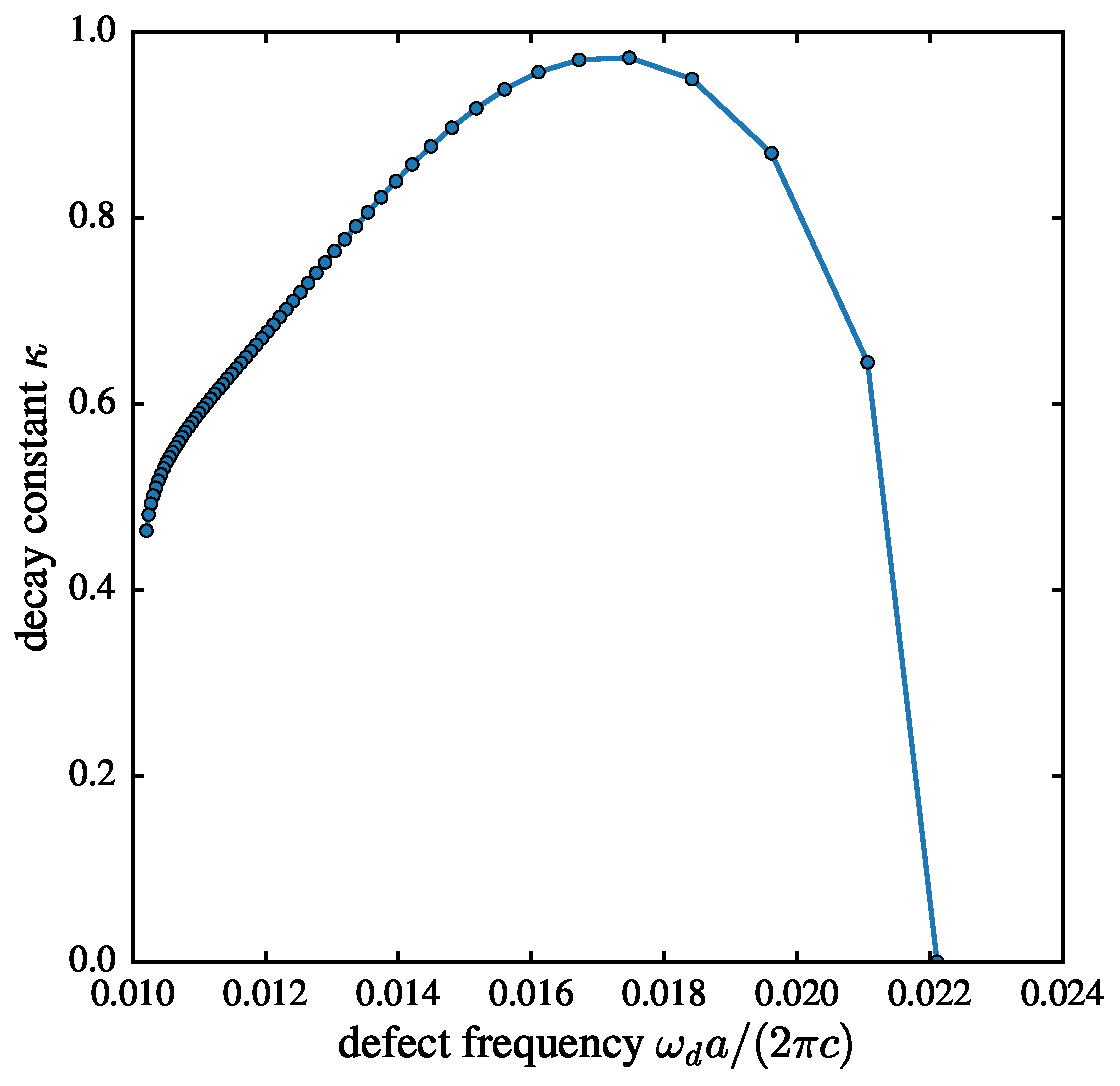
\includegraphics[width=0.5\textwidth]{3d-1}
\caption{\label{fig:3d} Decay constant calculated by fitting the electric field to a cosine oscillation bounded by a decaying exponential. The fit was calculated at each value of $d\varepsilon_2$, and is plotted against the defect frequency (for the first mode). This plot reveals the most highly localized mode occurs at the center of the gap.}
\end{figure*}


\end{document}